\section{Tree properties pt2}
\label{sec:tree_functions}

\begin{frame}
	\frametitle{Tree properties pt2}
	\begin{center}
		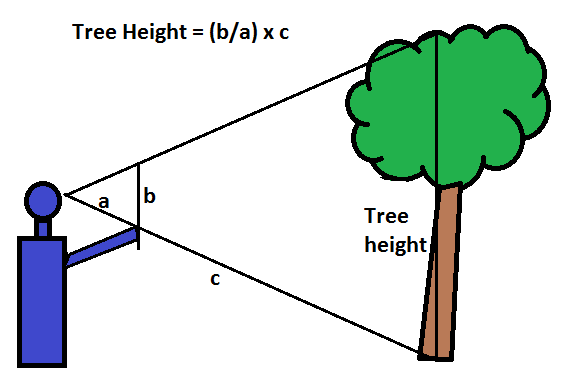
\includegraphics[width=0.6\textwidth]{figures/stick.png}\\
		\hspace*{15pt}\hbox{\scriptsize Image By:\thinspace{\itshape Edfrank01}}
		% https://commons.wikimedia.org/wiki/File:Stick_measurement.png
	\end{center}
\end{frame}

\begin{frame}
	\frametitle{Depth of a node}

	\begin{columns}
		\column{0.405\textwidth}
			\begin{tikzpicture}[
				level distance = 2.5em,
				level 1/.style={sibling distance=9em},
				level 2/.style={sibling distance=4.5em},
				level 3/.style={sibling distance=2.25em},
			]
			\node[ellipse] (t1) {root}
				child { node[ellipse]   {child 1}
					child { node[ellipse] {l1}}
				}
				child { node[ellipse]   {child 2}
					child { node[ellipse] {l2}}
					child { node[ellipse] {l3}}
					child { node[ellipse] {l4}}
				};
			\end{tikzpicture}
		\column{0.555\textwidth}
		\begin{itemize}
			\item The \textit{depth} of a \alert<5->{node} is the distance to the root.
				\pause
			\item So depth(root) = 0.
			\item And depth(l2) = 2.
				\pause
			\item The \textit{height} of a \alert<5->{tree} is the length of the longest path from root to leaf.
				\pause
			\item So the height of this tree is 3.
				\pause
			\item Note: Every book/author has their own definition of these things! Including our book :(
		\end{itemize}
	\end{columns}
	
\end{frame}

\begin{frame}
	\frametitle{Depth of a node}

	\begin{columns}
		\column{0.405\textwidth}
			\begin{tikzpicture}[
				level distance = 2.5em,
				level 1/.style={sibling distance=9em},
				level 2/.style={sibling distance=4.5em},
				level 3/.style={sibling distance=2.25em},
			]
			\node[ellipse] (t1) {root}
				child { node[ellipse]   {child 1}
					child { node[ellipse] {l1}}
				}
				child { node[ellipse]   {child 2}
					child { node[ellipse] {l2}}
					child { node[ellipse] {l3}}
					child { node[ellipse] {l4}}
				};
			\end{tikzpicture}
		\column{0.555\textwidth}
		\begin{questionblock}{Alternative definition for height}
			How can we also describe the tree height of a tree $T$?
			\pause
			\begin{enumerate}[A.]
				\item $\max\limits_{v\in T}({\textit{depth}(v)})-1$
				\item $\max\limits_{v\in T}({\textit{depth}(v)})$
				\item $\max\limits_{v\in T}({\textit{depth}(v)})+1$
			\end{enumerate}
		\end{questionblock}
	\end{columns}
	\pause
	\begin{answerblock}{A tree of height one}
		Remember that a tree of height one is just the root, which is at depth $0$. So it cannot be A or B.\\
		Then remember that depth is the distance, but height is the length of the path. These differ by 1, so C is the right
		answer.\\
		Our book uses $B$ :( 
	\end{answerblock}
\end{frame}

\begin{frame}
	\frametitle{An implementation}
	
	\begin{questionblock}{How do we implement this?}
		How can we implement such a tree structure?
	\end{questionblock}
	\pause
	\begin{answerblock}{Just like a DLL, only different}
		By using nodes that are \textit{linked} together to form a tree!
	\end{answerblock}
	\pause
	\begin{columns}[t]
		\column{0.535\textwidth}
	\lstinputlisting{code/tree.py}
			
		\column{0.505\textwidth}
	\lstinputlisting{code/treenode.py}
			
	\end{columns}
\end{frame}

\begin{frame}
	\frametitle{Now we can create functions!}
	\begin{questionblock}{Implementing functionality}
		What kind of \textit{programming paradigm} will we use to implement tree functions?
	\end{questionblock}
	\pause
	\begin{answerblock}{See the contents of this box}
		See the title of this box.
	\end{answerblock}
\end{frame}

\begin{frame}
	\frametitle{Node Depth}
		\begin{exampleblock}{Example: Node depth}
			Find the depth of a node is easy if we know the depth of the parent.
		\end{exampleblock}	
		\pause
		\lstinputlisting{code/nodedepth.py}
\end{frame}

\begin{frame}
	\frametitle{Tree Height}
		\begin{exampleblock}{Example: Tree height}
			The height of the tree is the max depth + 1! 	
		\end{exampleblock}	
		\pause
		\lstinputlisting{code/treeheight.py}
\end{frame}

\begin{frame}
	\frametitle{Getting all the leaves}
	\begin{questionblock}{It's autumn time}
		How can we get all the leaves from a tree?
	\end{questionblock}
		\pause
		\lstinputlisting{code/treeleaves.py}
\end{frame}

\begin{frame}
	\frametitle{The full ADT}
		\begin{alertblock}{A Tree ADT}
			Different implementations of trees, give you different ADTs.\\
			The book uses one which is \textit{position}-focused.\\
			The properties are always the same, just the functions and how to call them can be different.
		\end{alertblock}	
\end{frame}

\begin{frame}
	\frametitle{Alternative implementation}
		\begin{block}{An observation}
			Every node in a tree, is the root to a subtree!
		\end{block}	
		\pause
		\begin{columns}
			\column{0.455\textwidth}
				
			\begin{tikzpicture}[
				level distance = 2.5em,
				level 1/.style={sibling distance=9em},
				level 2/.style={sibling distance=4.5em},
				level 3/.style={sibling distance=2.25em},
			]
			\node[ellipse] (t1) {root}
				child { node[ellipse]   {child 1}
					child { node[ellipse] {l1}}
				}
				child { node[ellipse,onslide=<3>{draw=red}]   {child 2}
					child { node[ellipse] {\alert<3>{l2}}}
					child { node[ellipse] {\alert<3>{l3}}}
					child { node[ellipse] {\alert<3>{l4}}
						child { node[ellipse] {\alert<3>{l5}}}
						child { node[ellipse] {\alert<3>{l6}}}
					}
				};
			\end{tikzpicture}
			\pause
			\column{0.455\textwidth}
				\begin{exampleblock}{A subtree}
					In the example on the right, child 2 is the root of the subtree drawn in red.
				\end{exampleblock}	
		\end{columns}
\end{frame}

\begin{frame}
	\frametitle{Alternative implementation}
		\begin{block}{Thinking of all nodes as trees}
			By implementing it like this, we have no need for \texttt{TreeNode}s. All nodes are just \texttt{Tree}s!
		\end{block}	

		\lstinputlisting{code/tree_alt.py}
\end{frame}

\begin{frame}
	\frametitle{Alternative implementation: Tree Height}
	\begin{questionblock}{What do we do?}
		How do we determine the height in this set-up?
	\end{questionblock}
	\pause
	\lstinputlisting{code/tree_alt_height.py}
\end{frame}

\begin{frame}
	\frametitle{Why have one implementation over the other?}

	\begin{questionblock}{Which is better?}
		Which implementation should you use?
	\end{questionblock}
	\pause
	\begin{answerblock}{IT DEEP ENDS}
		It depends of course ;)\\
		What information do you need to store for your use case?
	\end{answerblock}
	
\end{frame}


